\documentclass{report}
\usepackage{hyperref}
\hypersetup{
    colorlinks=true,
    linkcolor=blue,
    filecolor=magenta,      
    urlcolor=cyan,
}
\usepackage{graphicx}
\graphicspath{ {imagenes/} }
\usepackage[utf8]{inputenc}
\makeatletter
\usepackage{color}
\definecolor{lightgray}{rgb}{0.95, 0.95, 0.95}
\definecolor{darkgray}{rgb}{0.4, 0.4, 0.4}
%\definecolor{purple}{rgb}{0.65, 0.12, 0.82}
\definecolor{editorGray}{rgb}{0.95, 0.95, 0.95}
\definecolor{editorOcher}{rgb}{1, 0.5, 0} % #FF7F00 -> rgb(239, 169, 0)
\definecolor{editorGreen}{rgb}{0, 0.5, 0} % #007C00 -> rgb(0, 124, 0)
\definecolor{orange}{rgb}{1,0.45,0.13}		
\definecolor{olive}{rgb}{0.17,0.59,0.20}
\definecolor{brown}{rgb}{0.69,0.31,0.31}
\definecolor{purple}{rgb}{0.38,0.18,0.81}
\definecolor{lightblue}{rgb}{0.1,0.57,0.7}
\definecolor{lightred}{rgb}{1,0.4,0.5}
\usepackage{upquote}
\usepackage{listings}
% CSS
\lstdefinelanguage{CSS}{
  keywords={color,background-image:,margin,padding,font,weight,display,position,top,left,right,bottom,list,style,border,size,white,space,min,width, transition:, transform:, transition-property, transition-duration, transition-timing-function},	
  sensitive=true,
  morecomment=[l]{//},
  morecomment=[s]{/*}{*/},
  morestring=[b]',
  morestring=[b]",
  alsoletter={:},
  alsodigit={-}
}

% JavaScript
\lstdefinelanguage{JavaScript}{
  morekeywords={typeof, new, true, false, catch, function, return, null, catch, switch, var, if, in, while, do, else, case, break},
  morecomment=[s]{/*}{*/},
  morecomment=[l]//,
  morestring=[b]",
  morestring=[b]'
}

\lstdefinelanguage{HTML5}{
  language=html,
  sensitive=true,	
  alsoletter={<>=-},	
  morecomment=[s]{<!-}{-->},
  tag=[s],
  otherkeywords={
  % General
  >,
  % Standard tags
	<!DOCTYPE,
  </html, <html, <head, <title, </title, <style, </style, <link, </head, <meta, />,
	% body
	</body, <body,
	% Divs
	</div, <div, </div>, 
	% Paragraphs
	</p, <p, </p>,
	% scripts
	</script, <script,
  % More tags...
  <canvas, /canvas>, <svg, <rect, <animateTransform, </rect>, </svg>, <video, <source, <iframe, </iframe>, </video>, <image, </image>, <header, </header, <article, </article
  },
  ndkeywords={
  % General
  =,
  % HTML attributes
  charset=, src=, id=, width=, height=, style=, type=, rel=, href=,
  % SVG attributes
  fill=, attributeName=, begin=, dur=, from=, to=, poster=, controls=, x=, y=, repeatCount=, xlink:href=,
  % properties
  margin:, padding:, background-image:, border:, top:, left:, position:, width:, height:, margin-top:, margin-bottom:, font-size:, line-height:,
	% CSS3 properties
  transform:, -moz-transform:, -webkit-transform:,
  animation:, -webkit-animation:,
  transition:,  transition-duration:, transition-property:, transition-timing-function:,
  }
}

\lstdefinestyle{htmlcssjs} {%
  % General design
%  backgroundcolor=\color{editorGray},
  basicstyle={\footnotesize\ttfamily},   
  frame=b,
  % line-numbers
  xleftmargin={0.75cm},
  numbers=left,
  stepnumber=1,
  firstnumber=1,
  numberfirstline=true,	
  % Code design
  identifierstyle=\color{black},
  keywordstyle=\color{blue}\bfseries,
  ndkeywordstyle=\color{editorGreen}\bfseries,
  stringstyle=\color{editorOcher}\ttfamily,
  commentstyle=\color{brown}\ttfamily,
  % Code
  language=HTML5,
  alsolanguage=JavaScript,
  alsodigit={.:;},	
  tabsize=2,
  showtabs=false,
  showspaces=false,
  showstringspaces=false,
  extendedchars=true,
  breaklines=true,
  % German umlauts
  literate=%
  {Ö}{{\"O}}1
  {Ä}{{\"A}}1
  {Ü}{{\"U}}1
  {ß}{{\ss}}1
  {ü}{{\"u}}1
  {ä}{{\"a}}1
  {ö}{{\"o}}1
}
%
\lstdefinestyle{py} {%
language=python,
literate=%
*{0}{{{\color{lightred}0}}}1
{1}{{{\color{lightred}1}}}1
{2}{{{\color{lightred}2}}}1
{3}{{{\color{lightred}3}}}1
{4}{{{\color{lightred}4}}}1
{5}{{{\color{lightred}5}}}1
{6}{{{\color{lightred}6}}}1
{7}{{{\color{lightred}7}}}1
{8}{{{\color{lightred}8}}}1
{9}{{{\color{lightred}9}}}1,
basicstyle=\footnotesize\ttfamily, % Standardschrift
numbers=left,               % Ort der Zeilennummern
%numberstyle=\tiny,          % Stil der Zeilennummern
%stepnumber=2,               % Abstand zwischen den Zeilennummern
numbersep=5pt,              % Abstand der Nummern zum Text
tabsize=4,                  % Groesse von Tabs
extendedchars=true,         %
breaklines=true,            % Zeilen werden Umgebrochen
keywordstyle=\color{blue}\bfseries,
frame=b,
commentstyle=\color{brown}\itshape,
stringstyle=\color{editorOcher}\ttfamily, % Farbe der String
showspaces=false,           % Leerzeichen anzeigen ?
showtabs=false,             % Tabs anzeigen ?
xleftmargin=17pt,
framexleftmargin=17pt,
framexrightmargin=5pt,
framexbottommargin=4pt,
%backgroundcolor=\color{lightgray},
showstringspaces=false,      % Leerzeichen in Strings anzeigen ?
}%
%
\makeatother

\begin{document}
\begin{titlepage}
    \centering
    {\bfseries\LARGE Universidad Politécnica Salesiana \par}
    \vspace{1cm}
    {\scshape\Large Ingeniería en Ciencias de la Computación \par}
    \vspace{3cm}
    {\scshape\Huge WEB SERVER \par}
    \vspace{1cm}
    {\center
\includegraphics[width=5cm, height=5cm]{ups1.png}\\}
    \vspace{1cm}
    {\itshape\Large Informe 03 \par}
    \vfill
    {\Large Autor: \par}
    {\Large Ricardo Romo \par}
    \vfill
    {\Large \today \par}
    \end{titlepage} 

    \section{Requisitos}
    Para crear un web server lo primero que necesitaremos son los módulos express, para arrancar el servidor,
    \textbf{handlebars} para los parciales y helpers
    \begin{enumerate}
      \item \textbf{Peraciales}: Templates o plantillas para los encabezados de las paginas html, a demás son el medio por las que se envían los datos
      \item \textbf{Helper}: Son funciones o ejecuciones del programa que se necesita corran en ciertas áreas cuando son llamadas
      
    \end{enumerate}
    
    \textbf{
    Instalacion Librerias:}
    \begin{enumerate}
     \item Iniciar npm con el comando \textbf{npm}
      \item Instalar la librería \textbf{express} con \textbf{npm install express --save}
      \item Instalar el módulo \textbf{handlebars} con \textbf{npm install hbs --save}
      \item Crear una carpeta llamada \textbf{hbs} y dentro de esta un documento llamado \textbf{helpers.js} los cuales almacenaran nuestros helpers para realizar funciones.
      \item Crear una carpeta \textbf{public } que es donde se almacenan a nuestros archivos estáticos que necesitara express
      \item Crear una carpeta llamada \textbf{views} y dentro de esta una carpeta llamada \textbf{parciales} y un archivo llamado \textbf{about.hbs} y uno llamado \textbf{home.hbs} que son nuestras páginas home y about con formato html
      \item Dentro de la carpeta parciales crear los archivos \textbf{footer.hbs} y \textbf{header.hbs} que son templates de las cabecera y pie de página de nuestras páginas html.
    \end{enumerate}
   
   \textbf{Express}
     \begin{center}
      
\includegraphics[scale=0.5]{exp.png}
     \end{center}
    \textbf{Handlebars}
     \begin{center}
      
\includegraphics[scale=0.1]{hbs.jpg}
     \end{center}
     \section{Server.js}
    
     \begin{enumerate}
       \item Para iniciar primero se instancian los módulos de \textbf{express} y hbs además se guarda el módulo de express dentro de una variable llamada \textbf{app}
       \lstinputlisting[firstline=1,lastline=2,style=htmlcssjs]{codigo/server.js}
       \item Se inicia la librería de hbs con require
       \item A demás de eso llamamos al puerto disponible que se nos asigna para poder levantar eln servidor
       \item Llamamos a nuestro archivo donde se almacenaran los helpers
       \lstinputlisting[firstline=3,lastline=5,style=htmlcssjs]{codigo/server.js}
      
    %-----------------------------------------------
    \item Utilizamos el comando \textbf{use} para establecer donde esta nuestra carpeta con nuestros archivos estáticos, además con el comando \textbf{\_\_dirname} establecemos la ruta de ejecución del servidor.
    \item  Utilizamos el comando \textbf{set} para establecer el manejo de los archivos html y especificamos que es con \textbf{hbs}
    \item el comando \textbf{hbs.registerPartials} nos ayuda a establecer donde almacenaremos nuestros templates.
    \lstinputlisting[firstline=7,lastline=9,style=htmlcssjs]{codigo/server.js}

    \item Con el comando \textbf{app.get} establecemos un pedido get a nuestro servidor, además con se debe de especificar la dirección a donde hacemos la petición, en este caso \textbf{\/} especifica la dirección raíz,
    \item con \textbf{res.render} establecemos los datos que deseamos enviar en este caso se enviara a nuestro archivo \textbf{home.hbs} los datos del nombre del usuario, la página y activación(pestañas en el navbar activables)
    \lstinputlisting[firstline=13,lastline=19,style=htmlcssjs]{codigo/server.js}
    \item Hacemos otra petición get pero con la dirección \textbf{\/about}
    \item Esta llamara a nuestro \textbf{about.hbs} y enviara los datos de página y que pestañas del navbar serán activables
  %-------------------------------------------------
  \lstinputlisting[firstline=22,lastline=27,style=htmlcssjs]{codigo/server.js}
  \item \textbf{app.listen()} levanta el puerto donde se dará el servicio.
  \lstinputlisting[firstline=30,lastline=32,style=htmlcssjs]{codigo/server.js}

\end{enumerate}

\section{helpers.js}
Ingresamos dentro del archivo \textbf{helpers.js} dentro de nuestra carpeta \textbf{hbs}
\begin{enumerate}
  \item se llama al módulo \textbf{hbs} antes ya instalado
  \lstinputlisting[firstline=1,lastline=1,style=htmlcssjs]{codigo/helpers.js}
  \item Con el comando \textbf{hbs.registerHelper()} se registra una función que se ejecutara en el html ('frontend') el cual recibe los parámetros del nombre de este helper y retorna un resultado
  \item En este caso nuestro herlper se llama \textbf{getAnio} y retorna el parámetro del año actual que uno se encuentra.
  \lstinputlisting[firstline=3,lastline=5,style=htmlcssjs]{codigo/helpers.js}
  \item Ahora se registraremos un nuevo template llamado \textbf{capitalizar } el cual recibirá un \textbf{string} y se encargara de dar un formato a cada palabra de esta, devolviendo el primer carácter de la palabra en mayúscula y los demás en minúscula
  \lstinputlisting[firstline=8,lastline=14,style=htmlcssjs]{codigo/helpers.js}
\end{enumerate}


  %------------------------

  \section{Parciales}
  Debido a q muchas páginas web utilizan los mismos encabezados, los parciales nos ayudan a tener cabeceras y pies de páginas ya estáticos y fáciles de llamar
  \subsection{header.hbs}
  Dentro del header tendremos nuestra cabecera la cual será el inicio del documento
  \lstinputlisting[firstline=1,lastline=12,style=htmlcssjs]{codigo/header.hbs}
  en nuestra cabecera podemos observar que para él la etiqueta del título llamamos al atributo \textbf{pagina} el cual se envía a través del server en la \textbf{petición get a nuestra dirección raíz}
  \\
  \textbf{Nota:}
  Además es importante recalcar que no estamos usando \textbf{bootstap} al contrario de esto estamos usando un derivado de este que \textbf{bootswatch} diseño \textbf{lux} el cual es amigable al llamar a través de un solo link y sin necesidad de crear carpetas secundarias con estilos \url{https://bootswatch.com/lux/}
  \\
  \textbf{Url guía componentes: } \url{https://bootswatch.com/lux/}
  \\
  \textbf{url para estilos css: } \url{https://bootswatch.com/4/lux/bootstrap.css}
  \subsection{footer.hbs}
  Dentro de \textbf{footer.hbs} tendremos lo que vendría siendo nuestro pie de pagina
  \lstinputlisting[firstline=1,lastline=17,style=htmlcssjs]{codigo/footer.hbs}
  \textbf{Nota:}
  Se puede observar cómo se llamar al helper \textbf{getAnio} el cual nos regresa nuestro año actual
  \subsection{navbar.hbs}
  Aquí instanciamos lo que vendría siendo la barra de opciones de nuestra página, este nav bar fue copiado de bootswatch el cual ya nos da con su diseño exclusivo.
  \\
  Además, podemos notar que enviamos las variables de activación para saber cuál pestaña u opción deberá prenderse a al estar en cierta página.
  \lstinputlisting[firstline=1,lastline=28,style=htmlcssjs]{codigo/navbar.hbs}
  \subsection{home.hbs}
  Esta página vendría siendo nuestra página principal al arrancar nuestro servidor y mostrarse en el navegador.
  \lstinputlisting[firstline=1,lastline=13,style=htmlcssjs]{codigo/navbar.hbs}
  \textbf{Nota:}
  Podemos apreciar como llamamos a nuestros templetes o parciales como nuestro \textbf{header,navbar y footer}, además podemos observar cómo llamamos a nuestro helper \textbf{capitalizar} y le enviamos el parámetro de \textbf{nombre} antes ya enviado por nuestro \textbf{server.js} a través de una petición get.
  \subsection{about.js}
  Así mismo podeos observar nuestro \textbf{about} el cual así mismo llamaremos a nuestros parciales o templetes para optimizar líneas de código html.
  \lstinputlisting[firstline=1,lastline=8,style=htmlcssjs]{codigo/about.hbs}
  %---------------------------
\section{Ejecucion}
\begin{enumerate}
  \item Primero ejecutamos el comando \textbf{node server.js}
  \begin{center}
    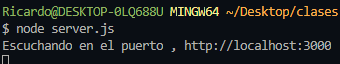
\includegraphics[scale=1]{eje1.PNG}
   \end{center}
  \item Luego nos dirijimos dentro del navegador a la direccion que nos muestra como resultado
  \begin{center}
    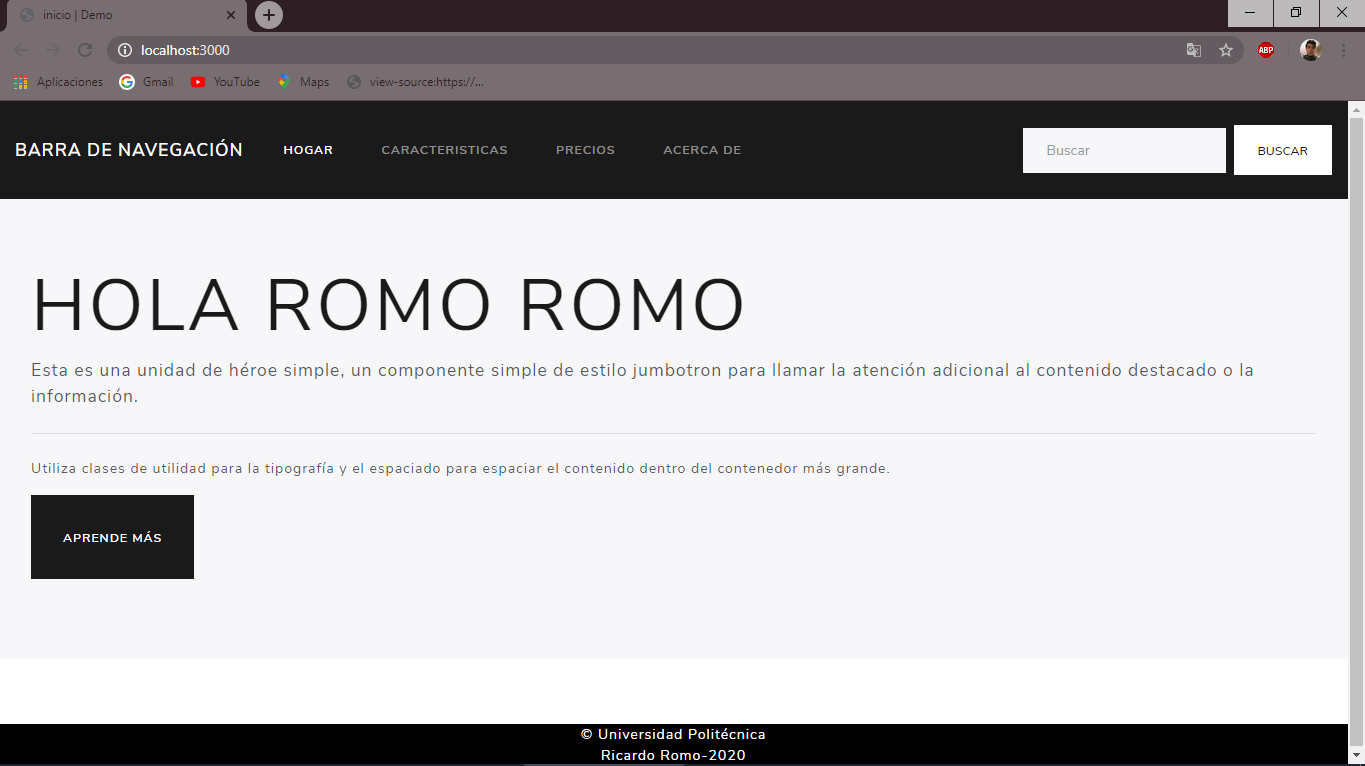
\includegraphics[scale=0.3]{eje2.PNG}
   \end{center}
  \item Al dar click en abaout podemos redirigirnos a la ventana about.hbs
  \begin{center}
    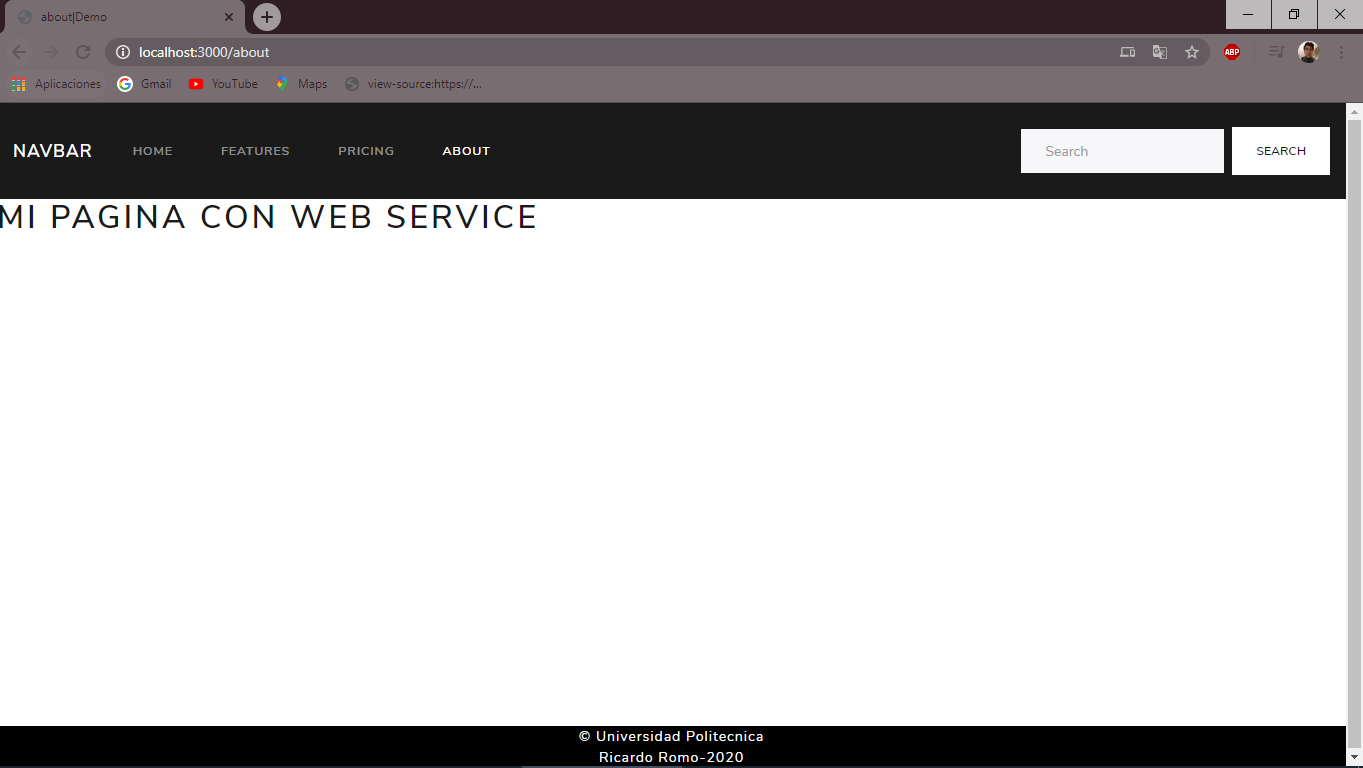
\includegraphics[scale=0.3]{eje3.PNG}
   \end{center}
  \item Y lo mismo al retornar al home
\end{enumerate}
\section{Repositorio}
\textbf{github:} \url{https://github.com/rromom/clases-web/tree/master/codigos/web_server}
\\
\textbf{heroku: }\url{https://romo-web-service.herokuapp.com/}

\end{document}